% This is "sig-alternate.tex" V2.0 May 2012
% This file should be compiled with V2.5 of "sig-alternate.cls" May 2012
%
% This example file demonstrates the use of the 'sig-alternate.cls'
% V2.5 LaTeX2e document class file. It is for those submitting
% articles to ACM Conference Proceedings WHO DO NOT WISH TO
% STRICTLY ADHERE TO THE SIGS (PUBS-BOARD-ENDORSED) STYLE.
% The 'sig-alternate.cls' file will produce a similar-looking,
% albeit, 'tighter' paper resulting in, invariably, fewer pages.
%
% ----------------------------------------------------------------------------------------------------------------
% This .tex file (and associated .cls V2.5) produces:
%       1) The Permission Statement
%       2) The Conference (location) Info information
%       3) The Copyright Line with ACM data
%       4) NO page numbers
%
% as against the acm_proc_article-sp.cls file which
% DOES NOT produce 1) thru' 3) above.
%
% Using 'sig-alternate.cls' you have control, however, from within
% the source .tex file, over both the CopyrightYear
% (defaulted to 200X) and the ACM Copyright Data
% (defaulted to X-XXXXX-XX-X/XX/XX).
% e.g.
% \CopyrightYear{2007} will cause 2007 to appear in the copyright line.
% \crdata{0-12345-67-8/90/12} will cause 0-12345-67-8/90/12 to appear in the copyright line.
%
% ---------------------------------------------------------------------------------------------------------------
% This .tex source is an example which *does* use
% the .bib file (from which the .bbl file % is produced).
% REMEMBER HOWEVER: After having produced the .bbl file,
% and prior to final submission, you *NEED* to 'insert'
% your .bbl file into your source .tex file so as to provide
% ONE 'self-contained' source file.
%
% ================= IF YOU HAVE QUESTIONS =======================
% Questions regarding the SIGS styles, SIGS policies and
% procedures, Conferences etc. should be sent to
% Adrienne Griscti (griscti@acm.org)
%
% Technical questions _only_ to
% Gerald Murray (murray@hq.acm.org)
% ===============================================================
%
% For tracking purposes - this is V2.0 - May 2012

\documentclass{sig-alternate}

\begin{document}
%
% --- Author Metadata here ---
\conferenceinfo{SIGIR}{'15, August 9-13, 2015, Santiago, Chile}
%\CopyrightYear{2007} % Allows default copyright year (20XX) to be over-ridden - IF NEED BE.
%\crdata{0-12345-67-8/90/01}  % Allows default copyright data (0-89791-88-6/97/05) to be over-ridden - IF NEED BE.
% --- End of Author Metadata ---

\title{ Facts behind the Words of a Patent Query
%\titlenote{(Produces the permission block, and
%copyright information). For use with
%SIG-ALTERNATE.CLS. Supported by ACM.}
}
\subtitle{Why Patent Prior-art Search Fails?
%\titlenote{A full version of this paper is available as
%\textit{Author's Guide to Preparing ACM SIG Proceedings Using
%\LaTeX$2_\epsilon$\ and BibTeX} at
%\texttt{www.acm.org/eaddress.htm}}
}
%
% You need the command \numberofauthors to handle the 'placement
% and alignment' of the authors beneath the title.
%
% For aesthetic reasons, we recommend 'three authors at a time'
% i.e. three 'name/affiliation blocks' be placed beneath the title.
%
% NOTE: You are NOT restricted in how many 'rows' of
% "name/affiliations" may appear. We just ask that you restrict
% the number of 'columns' to three.
%
% Because of the available 'opening page real-estate'
% we ask you to refrain from putting more than six authors
% (two rows with three columns) beneath the article title.
% More than six makes the first-page appear very cluttered indeed.
%
% Use the \alignauthor commands to handle the names
% and affiliations for an 'aesthetic maximum' of six authors.
% Add names, affiliations, addresses for
% the seventh etc. author(s) as the argument for the
% \additionalauthors command.
% These 'additional authors' will be output/set for you
% without further effort on your part as the last section in
% the body of your article BEFORE References or any Appendices.

%\numberofauthors{8} %  in this sample file, there are a *total*
% of EIGHT authors. SIX appear on the 'first-page' (for formatting
% reasons) and the remaining two appear in the \additionalauthors section.
%
\author{
% You can go ahead and credit any number of authors here,
% e.g. one 'row of three' or two rows (consisting of one row of three
% and a second row of one, two or three).
%
% The command \alignauthor (no curly braces needed) should
% precede each author name, affiliation/snail-mail address and
% e-mail address. Additionally, tag each line of
% affiliation/address with \affaddr, and tag the
% e-mail address with \email.
%
% 1st. author
%\alignauthor
%Ben Trovato\titlenote{Dr.~Trovato insisted his name be first.}\\
%       \affaddr{Institute for Clarity in Documentation}\\
%       \affaddr{1932 Wallamaloo Lane}\\
%       \affaddr{Wallamaloo, New Zealand}\\
%       \email{trovato@corporation.com}
% 2nd. author
%\alignauthor
%G.K.M. Tobin\titlenote{The secretary disavows
%any knowledge of this author's actions.}\\
%       \affaddr{Institute for Clarity in Documentation}\\
%       \affaddr{P.O. Box 1212}\\
%       \affaddr{Dublin, Ohio 43017-6221}\\
%       \email{webmaster@marysville-ohio.com}
%% 3rd. author
%\alignauthor Lars Th{\o}rv{\"a}ld\titlenote{This author is the
%one who did all the really hard work.}\\
%       \affaddr{The Th{\o}rv{\"a}ld Group}\\
%       \affaddr{1 Th{\o}rv{\"a}ld Circle}\\
%       \affaddr{Hekla, Iceland}\\
%       \email{larst@affiliation.org}
%\and  % use '\and' if you need 'another row' of author names
% 4th. author
%\alignauthor Lawrence P. Leipuner\\
%       \affaddr{Brookhaven Laboratories}\\
%       \affaddr{Brookhaven National Lab}\\
%       \affaddr{P.O. Box 5000}\\
%       \email{lleipuner@researchlabs.org}
% 5th. author
%\alignauthor Sean Fogarty\\
%       \affaddr{NASA Ames Research Center}\\
%       \affaddr{Moffett Field}\\
%       \affaddr{California 94035}\\
%       \email{fogartys@amesres.org}
%% 6th. author
%\alignauthor Charles Palmer\\
%       \affaddr{Palmer Research Laboratories}\\
%       \affaddr{8600 Datapoint Drive}\\
%       \affaddr{San Antonio, Texas 78229}\\
%       \email{cpalmer@prl.com}
}
% There's nothing stopping you putting the seventh, eighth, etc.
% author on the opening page (as the 'third row') but we ask,
% for aesthetic reasons that you place these 'additional authors'
% in the \additional authors block, viz.
%\additionalauthors{Additional authors: John Smith (The Th{\o}rv{\"a}ld Group,
%email: {\texttt{jsmith@affiliation.org}}) and Julius P.~Kumquat
%(The Kumquat Consortium, email: {\texttt{jpkumquat@consortium.net}}).}
\date{30 July 1999}
% Just remember to make sure that the TOTAL number of authors
% is the number that will appear on the first page PLUS the
% number that will appear in the \additionalauthors section.

\maketitle
\begin{abstract}

\end{abstract}

% A category with the (minimum) three required fields
\category{H.3.3}{Information Search and Retrieval}{Query Formulation}
%A category including the fourth, optional field follows...
%\category{D.2.8}{Software Engineering}{Metrics}[complexity measures, performance measures]

\terms{Theory}

\keywords{patent search, Query Reformulation, Data Analysis}

\section{Introduction}

\section{Baseline}

\section{Term Analysis}
The main complain about patent search is insufficient match between the content of patent queries and relevant
patents\cite{magdy2012toward, mahdabi2013leveraging}. However, our analyses showed that only \%20 overlap is sufficient for the system to retrieve a relevant or non-relevant patent at top-100 and except for few queries, non-retrieved relevant patents had enough matched term with the query. So, we start our experiments with term analysis for patent query and retrieved documents. 

\subsection{Discriminative Words}
For our initial experiments, we identified the {\em discriminative words} by positive scoring the words in relevant documents and negative scoring the irrelevant one. 
\begin{equation}
score(t,Q)=Rel(t)-Irr(t) 
 \label{eq:score}
\end{equation}
\begin{displaymath}t\in \lbrace \mbox{terms in top-100 retrieved documents}\rbrace\end{displaymath}
Where $ Rel(t) $ is the average term frequency in retrieved relevant patents and $ Irr(t) $ is the average term frequency in retrieved irrelevant patents. Words with a positive score consider {\em useful terms} since they are more frequent in relevant patents. 

Surprisingly, we could not find any correlation between the percentage of {\em useful terms} and the performance. We expected a higher performance for the queries with more {\em useful terms}. 

\subsubsection{Optimal RF\protect\footnote{Relevance Feedback} Query Formulation}
We hypothesize that a query formulated by {\em useful terms} is optimal since they are all frequent in relevant patents and rare in irrelevant ones. Table \ref{tab:optquery} compares the performance for baseline where the query is the full patent query both weighted and unweighed with the performance for optimal RF query weighted with the score of each term(formula \ref{eq:score}) and unweighed. 

\begin{table}[htpb]
  \begin{center}
   \caption{.}
  \input table/optquery.tex   
  \label{tab:optquery}
  \end{center}  
\end{table}

It can be seen that `MAP' jumps from 0.1618 to \textbf{0.5075} which is about \%35 increase. Fig. ... shows 

%\begin{figure}[htpb]
%\centering
%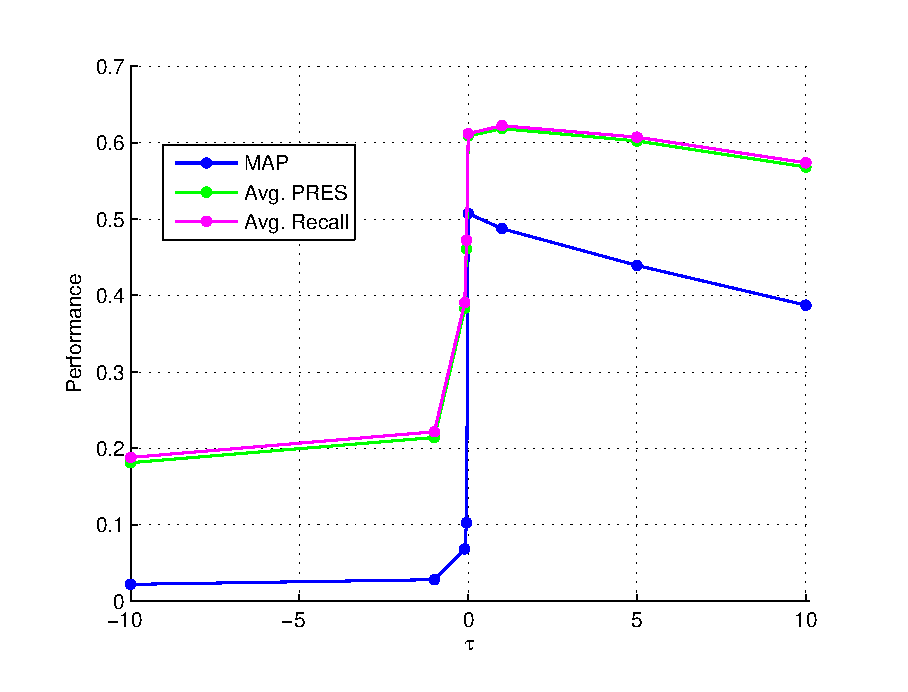
\epsfig{file=figs/extended-optquery-tau.eps, height=2in, width=3.1in}
%\caption{A sample black and white graphic (.eps format).}
%\end{figure}

%\begin{figure}[htpb]
%\begin{center}
%\begin{minipage}{\linewidth/2}
%%\begin{center}
%%\vspace{-1mm}
%%\quad
%%\begin{subfigure}{0.19\linewidth}
%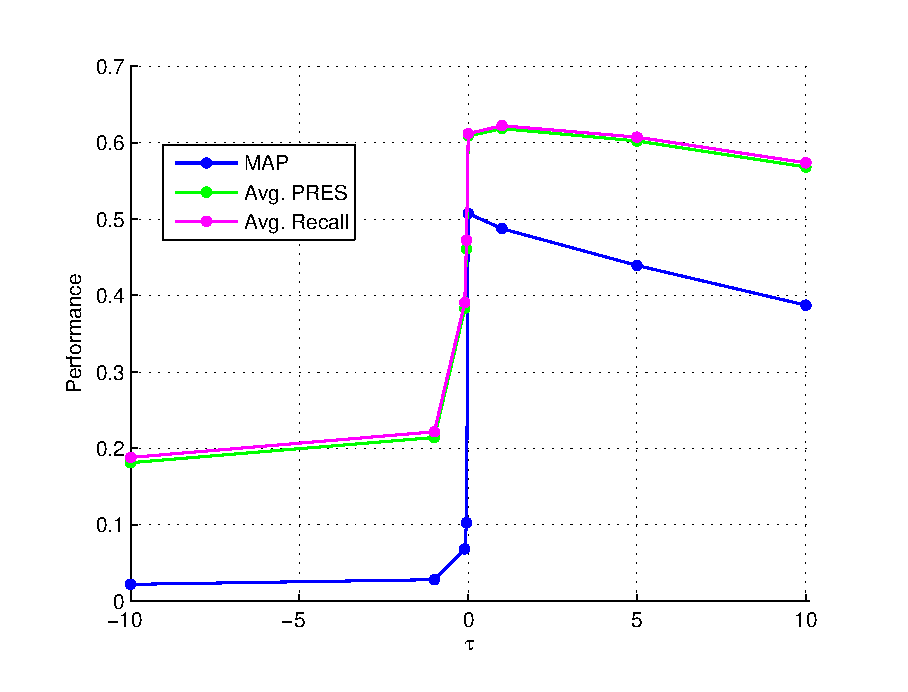
\includegraphics[width=0.8\linewidth]{figs/extended-optquery-tau.eps}
%%\\ \begin{center}(b)\end{center}%\caption{}
%%\label{fig:mom0}
%% \end{subfigure}%
%\end{minipage}
%\hspace{7mm}
%\begin{minipage}{\linewidth/2}
%%\qquad
%%\begin{subfigure}{0.52\linewidth}
%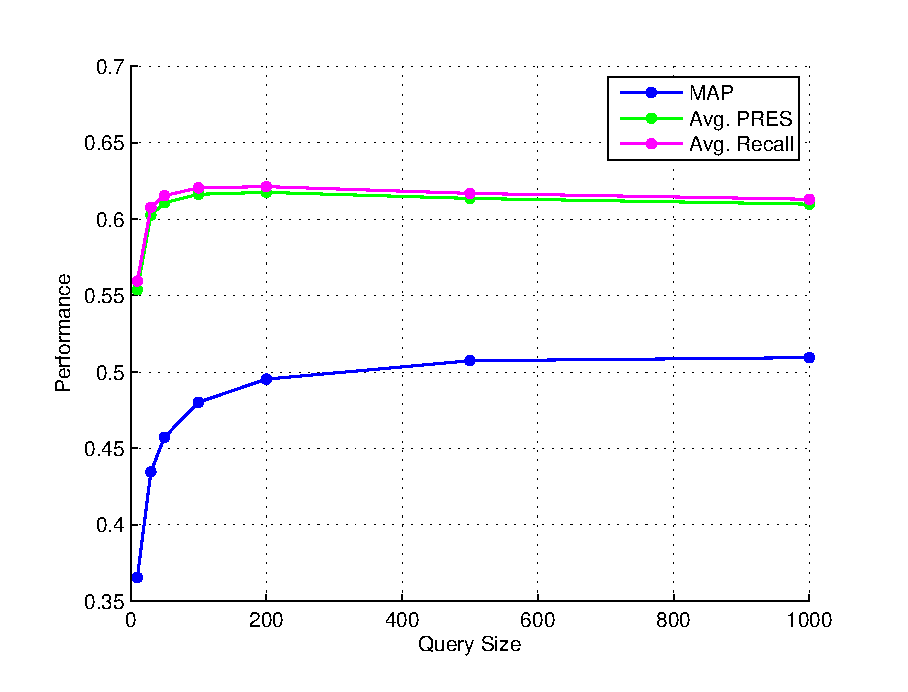
\includegraphics[width=0.80\linewidth]{figs/opt-query-qsize.eps}
%%\\ \begin{center}(b)\end{center}%\caption{}
%%\label{fig:mom00}
%% \end{subfigure}%
%%\end{center}
%\end{minipage}
%\vspace{3mm}\\
%(a) \hspace{30mm}(b)
%%\vspace{-1mm}
%\caption{\footnotesize
%Collision of masses $M_1$ and $M_2$ with velocities $V_1$ and $V_2$ and momenta $P_1$ and $P_2$.
%(a) Collision happens if and only if $V_1>V_2$. (b) Corresponding Bayesian network. The non-filled and filled Filled circles represent stochastic and deterministic random variables respectively.}
%\label{fig:mom2}
%\vspace{-4mm}
%
%\end{center}
%\end{figure}


\begin{figure}
\centering
\subfloat[]{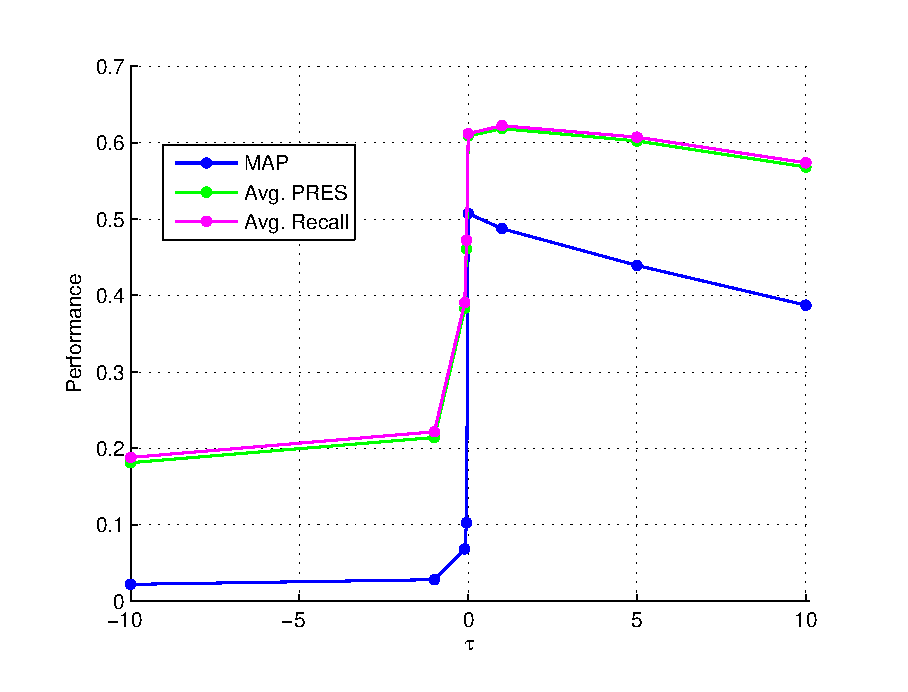
\includegraphics[width=3.1in]{figs/extended-optquery-tau.eps}} 
\subfloat[]{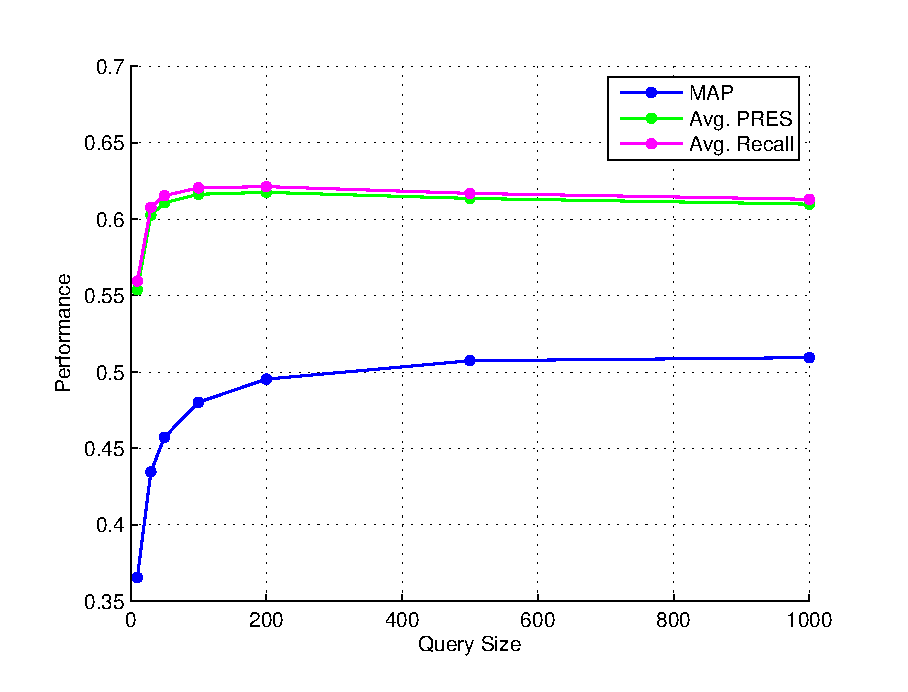
\includegraphics[width=3.1in]{figs/opt-query-qsize.eps}}
\caption{Potential for 0.5 V bias.} 
\label{fig:EcUND} 
\end{figure} 

%\begin{figure}[htpb]
%\centering
%\begin{subfigure}[htpb]{.50\linewidth}
%\centering
%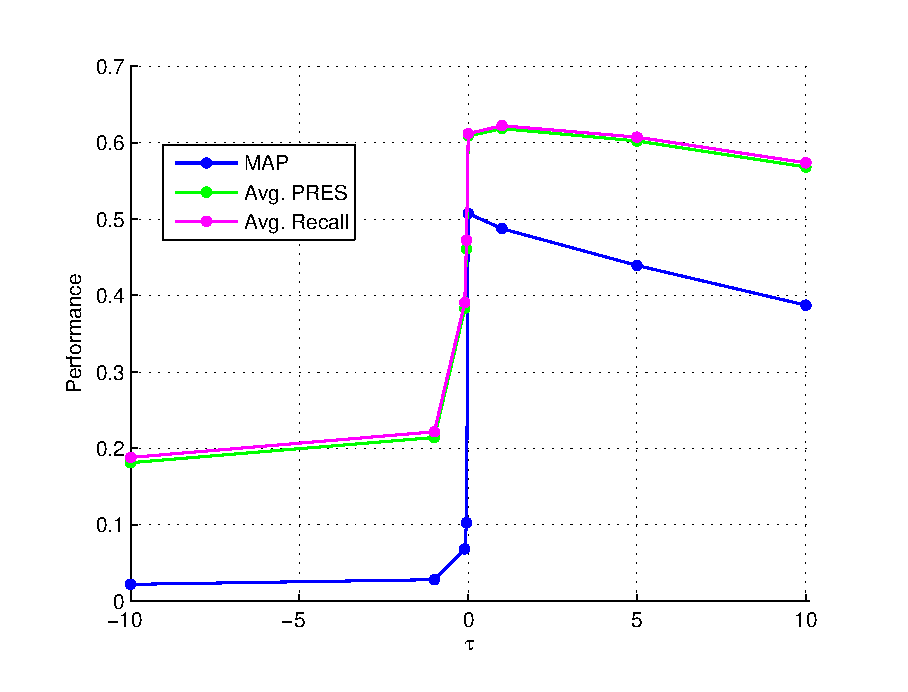
\includegraphics[width=1\textwidth,height=52mm]{figs/extended-optquery-tau.eps}
%\caption{Optimal RF query performance versus the score threshold to select optimal query terms.}%
%\label{fig:thresh1}
%\end{subfigure}%
%\centering
%\begin{subfigure}[htpb]{.5\linewidth}
%\centering
%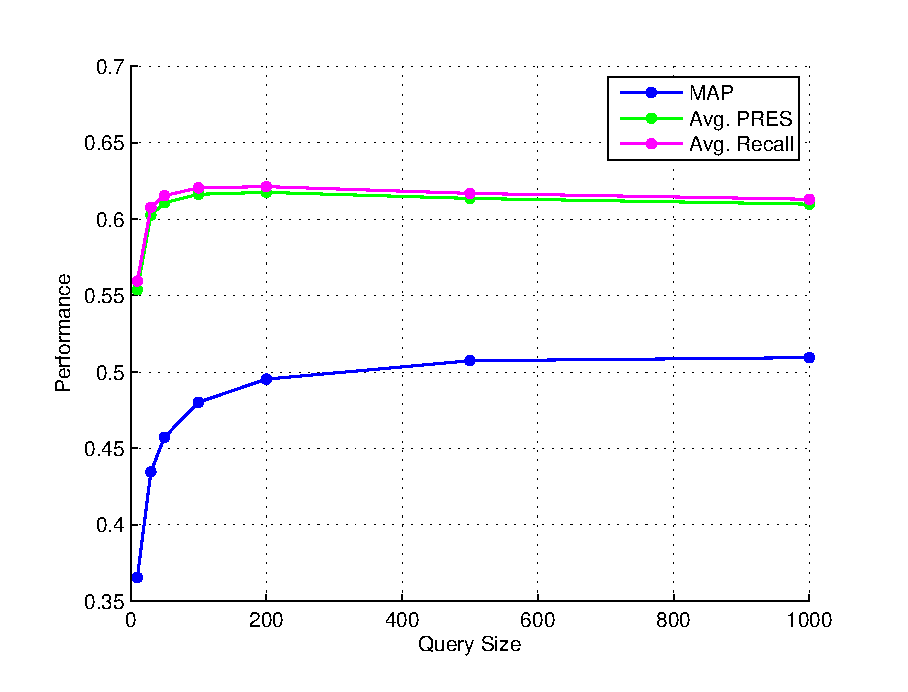
\includegraphics[width=1\textwidth,height=52mm]{figs/opt-query-qsize.eps}
%\caption{Optimal RF query performance versus the query size.}
%\label{fig:qsize}
%\end{subfigure}\\[1ex]%
%%\begin{subfigure}[htpb]{.5\linewidth}
%%\centering
%%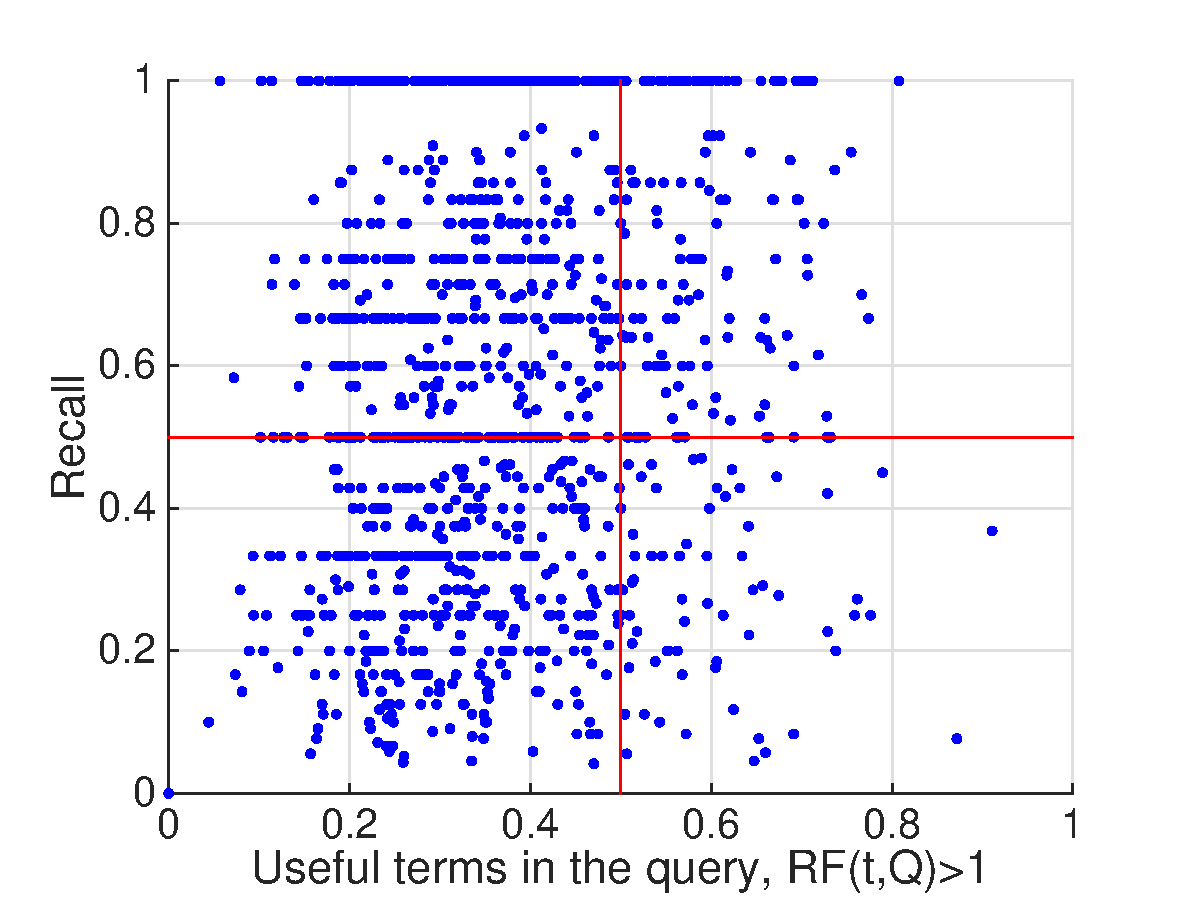
\includegraphics[width=1\textwidth,height=52mm]{figs/greaterthan1-r.eps}
%%\caption{Useful terms: $ score(t_{i})>1 $}
%%\label{fig:greater1r}
%%\end{subfigure}%
%%\centering
%%\begin{subfigure}[htpb]{.5\linewidth}
%%\centering
%%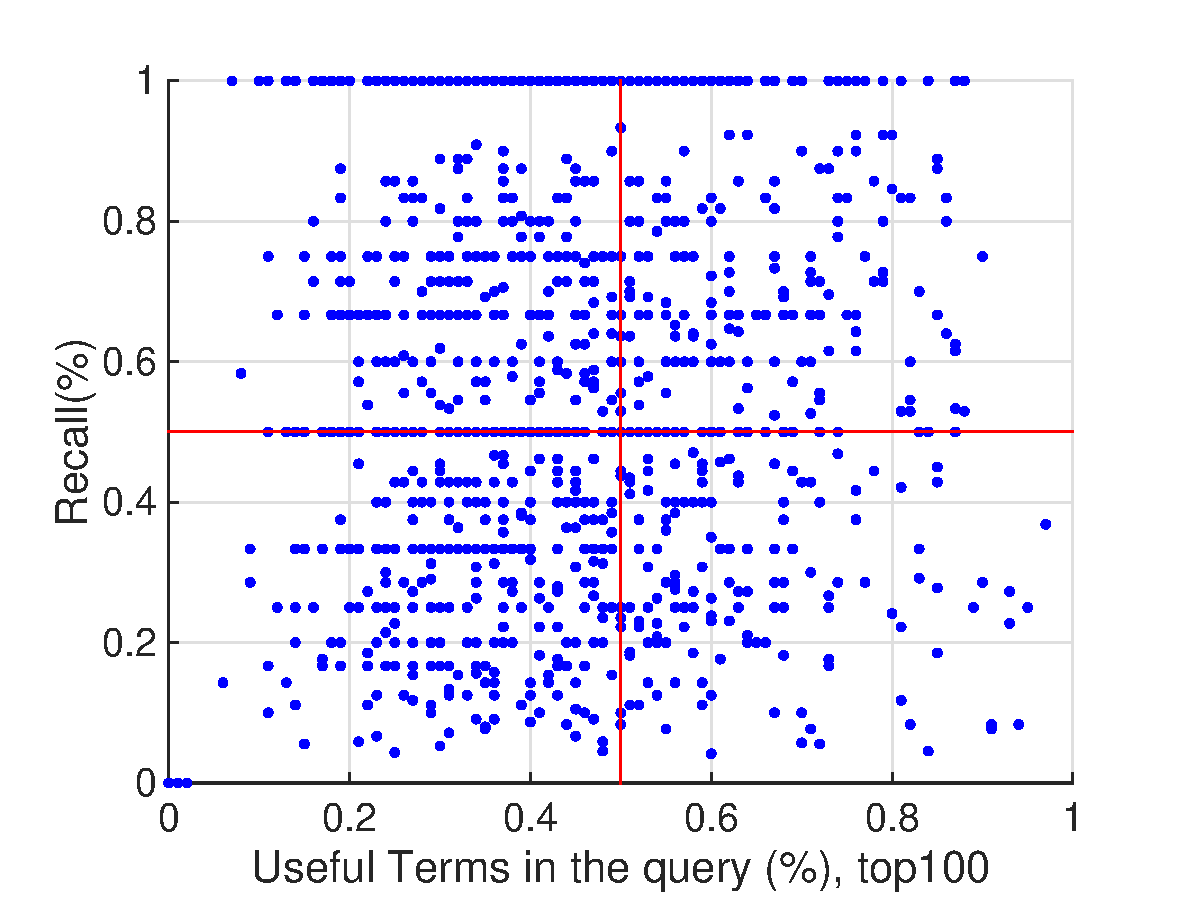
\includegraphics[width=1\textwidth,height=52mm]{figs/top100-r.eps}
%%\caption{Useful terms: top 100 high-scored terms}
%%\label{fig:top100r}
%%\end{subfigure}\\[1ex]%
%%\begin{subfigure}[htpb]{.5\linewidth}
%%\centering
%%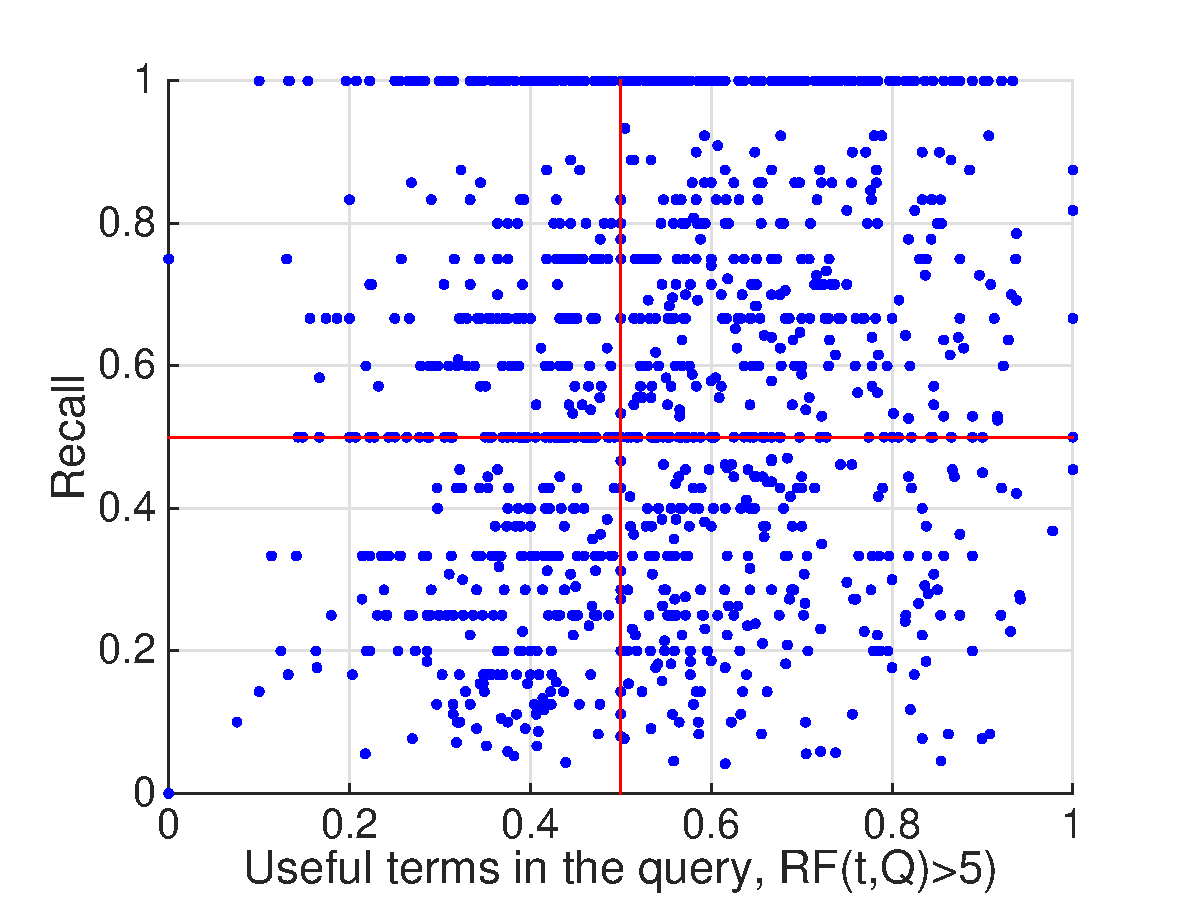
\includegraphics[width=1\textwidth,height=52mm]{figs/greaterthan5-r.eps}
%%\caption{Useful terms: $ score(t_{i})>5 $}
%%\label{fig:greater1r}
%%\end{subfigure}%
%%\centering
%%\begin{subfigure}[htpb]{.5\linewidth}
%%\centering
%%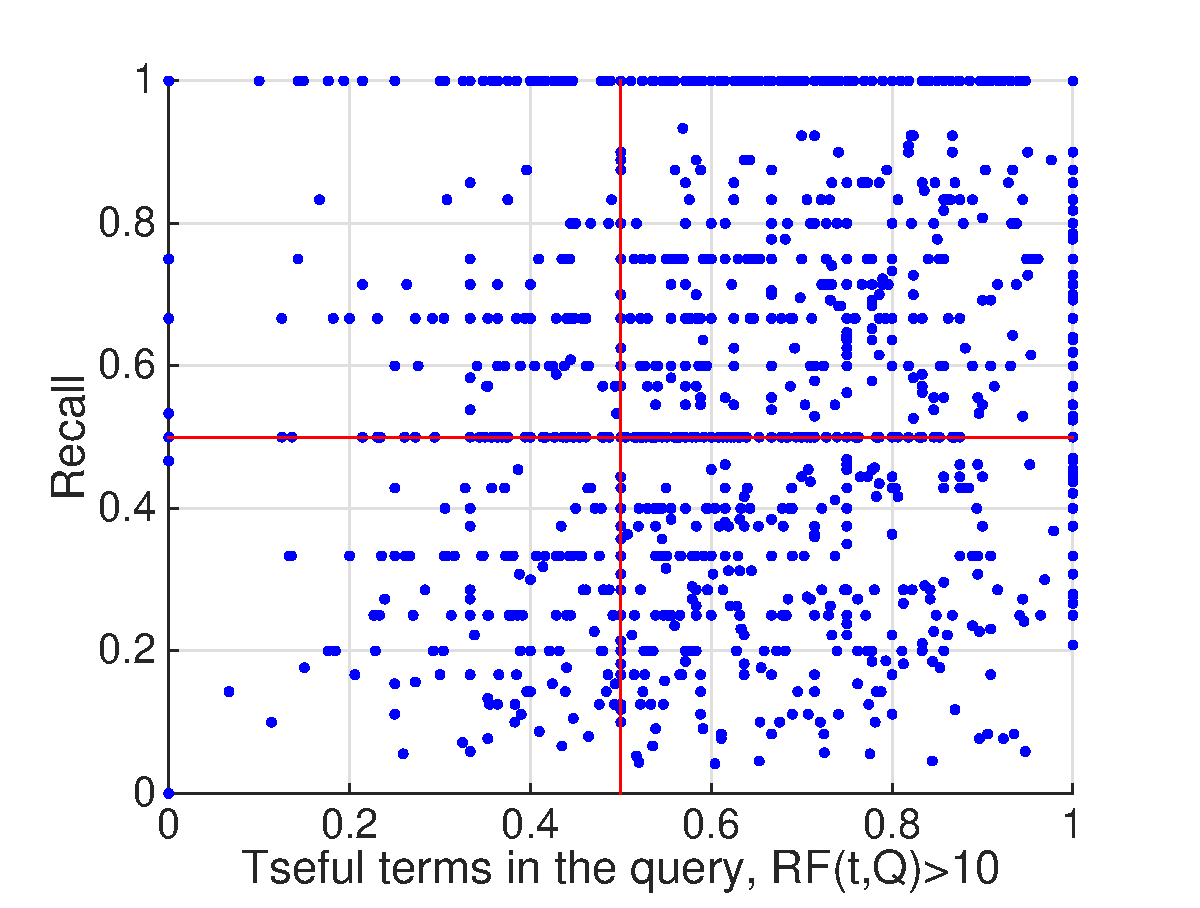
\includegraphics[width=1\textwidth,height=52mm]{figs/greaterthan10-r.eps}
%%\caption{Useful terms: $ score(t_{i})>10 $}
%%\label{fig:greater0r}
%%\end{subfigure}
%\caption{Comparing the optimal query performance versus the $score_{RF}$ threshold and query size(weight:1).}
%\label{fig:querysizeandthreshold}
%\end{figure}

\subsubsection{Query Reduction by RF}

\subsection{What did not Work}

\subsubsection{Pseudo Relevance Feedback}

\subsubsection{Identify the Noisy Words}

\subsection{Improvement by Minimum User Effort}

\section{Related Work}

\section{Conclusions}

%\end{document}  % This is where a 'short' article might terminate

%ACKNOWLEDGMENTS are optional
\section{Acknowledgments}


%
% The following two commands are all you need in the
% initial runs of your .tex file to
% produce the bibliography for the citations in your paper.
\bibliographystyle{abbrv}
\bibliography{sigproc}  % sigproc.bib is the name of the Bibliography in this case
% You must have a proper ".bib" file
%  and remember to run:
% latex bibtex latex latex
% to resolve all references
%
% ACM needs 'a single self-contained file'!
%
%APPENDICES are optional
%\balancecolumns
%\appendix
%%Appendix A
%\section{Headings in Appendices}
%The rules about hierarchical headings discussed above for
%the body of the article are different in the appendices.
%In the \textbf{appendix} environment, the command
%\textbf{section} is used to
%indicate the start of each Appendix, with alphabetic order
%designation (i.e. the first is A, the second B, etc.) and
%a title (if you include one).  So, if you need
%hierarchical structure
%\textit{within} an Appendix, start with \textbf{subsection} as the
%highest level. Here is an outline of the body of this
%document in Appendix-appropriate form:
%\subsection{Introduction}
%\subsection{The Body of the Paper}
%\subsubsection{Type Changes and  Special Characters}
%\subsubsection{Math Equations}
%\paragraph{Inline (In-text) Equations}
%\paragraph{Display Equations}
%\subsubsection{Citations}
%\subsubsection{Tables}
%\subsubsection{Figures}
%\subsubsection{Theorem-like Constructs}
%\subsubsection*{A Caveat for the \TeX\ Expert}
%\subsection{Conclusions}
%\subsection{Acknowledgments}
%\subsection{Additional Authors}
%This section is inserted by \LaTeX; you do not insert it.
%You just add the names and information in the
%\texttt{{\char'134}additionalauthors} command at the start
%of the document.
%\subsection{References}
%Generated by bibtex from your ~.bib file.  Run latex,
%then bibtex, then latex twice (to resolve references)
%to create the ~.bbl file.  Insert that ~.bbl file into
%the .tex source file and comment out
%the command \texttt{{\char'134}thebibliography}.
%% This next section command marks the start of
%% Appendix B, and does not continue the present hierarchy
%\section{More Help for the Hardy}
%The sig-alternate.cls file itself is chock-full of succinct
%and helpful comments.  If you consider yourself a moderately
%experienced to expert user of \LaTeX, you may find reading
%it useful but please remember not to change it.
%\balancecolumns % GM June 2007
% That's all folks!



\end{document}
